%! TeX program = lualatex
\documentclass[a4paper]{article} 

% packages
\usepackage{microtype}      % Slightly tweak font spacing for aesthetics
\usepackage[english]{babel} % Language hyphenation and typographical rules
\usepackage{changepage}     % adjust margins on the fly

\usepackage[final, colorlinks = true, urlcolor = black, linkcolor = black, citecolor = black]{hyperref} 
\usepackage{fontspec}
% \setmainfont{EB Garamond}
% \setmonofont[Scale=MatchLowercase]{Deja Vu Sans Mono}

\setmainfont{EB Garamond}[
    Ligatures=TeX,
    Numbers=OldStyle
]

% Fallback font (for missing characters)
\setmainfont{EB Garamond}[
    % Ligatures=TeX,
    % Numbers=OldStyle
]

\newfontfamily{\emojifont}{Noto Color Emoji}[Renderer=Harfbuzz]

% Monospace font configuration
\setmonofont[Scale=MatchLowercase]{DejaVu Sans Mono}

\usepackage[backend=biber, style=numeric, date=iso, urldate=iso]{biblatex}
\addbibresource{references.bib}
\DeclareFieldFormat{urldate}{Accessed on: #1}

\usepackage{minted}
\usemintedstyle{algol_nu}
\usepackage{xcolor}

\usepackage{pgfplots}
\pgfplotsset{width=\textwidth,compat=1.9}

\usepackage{caption}
\newenvironment{code}{\captionsetup{type=listing}}{}
\captionsetup[listing]{skip=0pt}
\setlength{\abovecaptionskip}{5pt}
\setlength{\belowcaptionskip}{5pt}

\usepackage[yyyymmdd]{datetime}
\renewcommand{\dateseparator}{--}

\usepackage{titlesec}
% \titleformat{\section}{\LARGE\bfseries}{}{}{}[\titlerule]
% \titleformat{\subsection}{\Large\bfseries}{}{0em}{}
% \titlespacing{\subsection}{0em}{-0.7em}{0em}
%
% \titleformat{\subsubsection}{\large\bfseries}{}{0em}{$\bullet$ }
% \titlespacing{\subsubsection}{1em}{-0.7em}{0em}

% margins
\addtolength{\hoffset}{-2.25cm}
\addtolength{\textwidth}{4.5cm}
\addtolength{\voffset}{-3.25cm}
\addtolength{\textheight}{5cm}
\setlength{\parskip}{0pt}
\setlength{\parindent}{0in}
% \setcounter{secnumdepth}{0}

\begin{document}
\hrule \medskip
\begin{minipage}{0.295\textwidth} 
    \raggedright
    \footnotesize 
    \begin{tabular}{@{}l l}
        Name: & Andrew Hayes \\
        Student ID: & 21321503 \\
        E-mail: & \href{mailto://a.hayes18@universityofgalway.ie}{\texttt{a.hayes18@universityofgalway.ie}} \\
    \end{tabular}
\end{minipage}
\begin{minipage}{0.4\textwidth} 
    \centering 
    \vspace{0.4em}
    \LARGE
    \textsc{ct420} \\ 
\end{minipage}
\begin{minipage}{0.295\textwidth} 
    \raggedleft
    \today
\end{minipage}
\medskip\hrule 
\begin{center}
    \normalsize
    Assignment 2: POSIX Programming \& Benchmarking
\end{center}
\hrule
\medskip

\section{Host Environment}
For my host environment, I chose to run Ubuntu Server 24.04.2 LTS using a VirtualBox hypervisor.
I chose this operating system as I have sufficient Linux experience to feel confident using an operating system with no graphical interface (as opposed to Ubuntu Desktop), and the absence of a GUI means a smaller ISO file, memory footprint, \& CPU footprint.
I chose Ubuntu specifically because it's a Linux system with which I have previous experience, and is well-document with plenty of packages available to install if needs be.
Ubuntu also makes it easy to install the \verb|PREEMPT_RT| patches, which transform the standard Linux kernel into a fully preemptible, real-time kernel, which I felt was more suitable for this assignment, as the standard Linux kernel is not suitable for a hard real-time system due to its lack of preemption.

\begin{figure}[H]
    \centering
    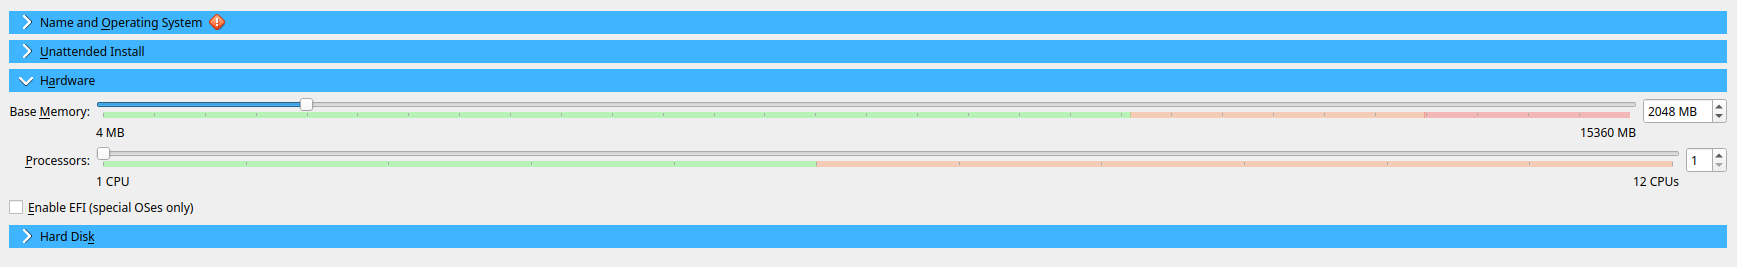
\includegraphics[width=\textwidth]{./images/hardware.png}
    \caption{Virtual machine hardware configuration}
\end{figure}

I set the virtual machine to have a single CPU and set the amount of RAM to 2048MB which is the recommended minimum for Ubuntu Server\supercite{ubuntu_server_installation}.
I left the hard disk size at the default of 25GB as I saw no reason to change it.
The real-time kernel with the \verb|PREEMPT_RT| patches installed is available with Ubuntu Pro, which is free for personal use.
After setting up an Ubuntu Pro account, I enabled the real-time kernel using the \mintinline{bash}{pro} command.

\begin{figure}[H]
    \centering
    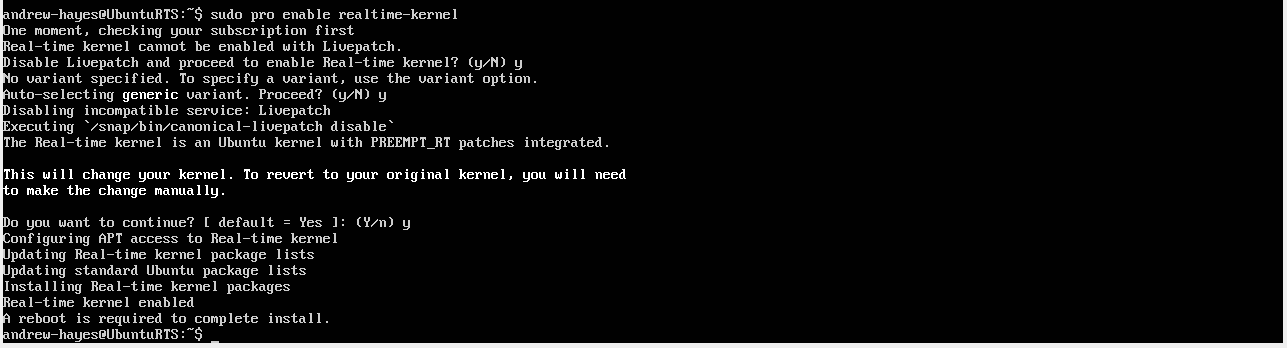
\includegraphics[width=\textwidth]{./images/proenable.png}
    \caption{Enabling the real-time kernel with the \mintinline{bash}{pro} command}
\end{figure}

Finally, I transferred over the following C file (taken from the lecture slides) via \mintinline{shell}{scp}\supercite{scp} to the virtual machine to get the clock resolution, which is 1 nanosecond:
\begin{code}
\begin{minted}[linenos, breaklines, frame=single]{C}
#include<unistd.h>
#include<time.h>
#include <stdio.h>

int main(){
    struct timespec clock_res;
    int stat;
    stat=clock_getres(CLOCK_REALTIME, &clock_res);
    printf("Clock resolution is %d seconds, %ld nanoseconds\n",clock_res.tv_sec,clock_res.tv_nsec);
    return 0;
}
\end{minted}
\end{code}

\begin{figure}[H]
    \centering
    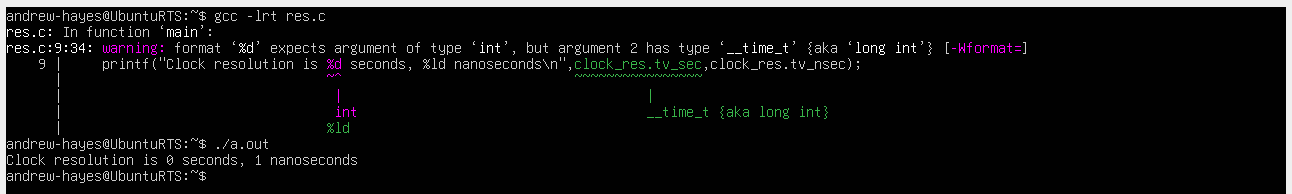
\includegraphics[width=\textwidth]{./images/clockres.png}
    \caption{Getting the clock resolution of the virtual machine}
\end{figure}

\section{Benchmarking Code}
I combined the provided benchmarking programs \verb|bm1.c| and \verb|bm2.c| into a single file, and added logic to benchmark the \mintinline{c}{usleep()} function as well as outputting the relevant data to CSV files.
Additionally, I updated the \mintinline{c}{#define ITERATIONS} constant to have value \mintinline{c}{10000} and I also tweaked the \mintinline{c}{while (!timer_expired)} loop to sleep for 100 nanoseconds in-between evaluations of the loop condition, as I found that the ``busy waiting'' was greatly slowing down the program when I ran it on my virtual machine.
There is a potential drawback to this however:
adding the \mintinline{c}{nanosleep()} to the while loop could artificially introduce a delay into obtaining the data, as there could be a maximum delay of 100 nanoseconds before the timer is registered as expired.
However, since the busy wait was artificially increasing the runtime, and much more so than the version with the sleep, it too would introduce delay, and much more than the modified version, as the modified version ran around 10 times more quickly.
Therefore, while this modification could potentially introduce noise to the data collected for the interval timer benchmark, it introduces less error than the busy wait, so I decided to include the modification.

\begin{code}
\inputminted[linenos, breaklines, frame=single]{C}{../code/benchmarks/merged.c}
\caption{\texttt{merged.c}}
\end{code}

\section{CPU \& Data-Intensive Applications}
To develop my CPU \& data-intensive programs, I chose to use Python for ease of development.
I chose \mintinline{shell}{htop}\supercite{htop} as my resource-monitoring tool as I have often used it in the past, it has easy to read \& understand output, and shows you exactly what proportion of the CPU \& memory is in use at that time.
It also allows you to list processes by CPU consumption or memory consumption which is a useful option to have for this assignment.

\begin{code}
\inputminted[linenos, breaklines, frame=single]{python}{../code/stressers/stress_cpu.py}
\caption{\texttt{stress\_cpu.py}}
\end{code}

\begin{figure}[H]
    \centering
    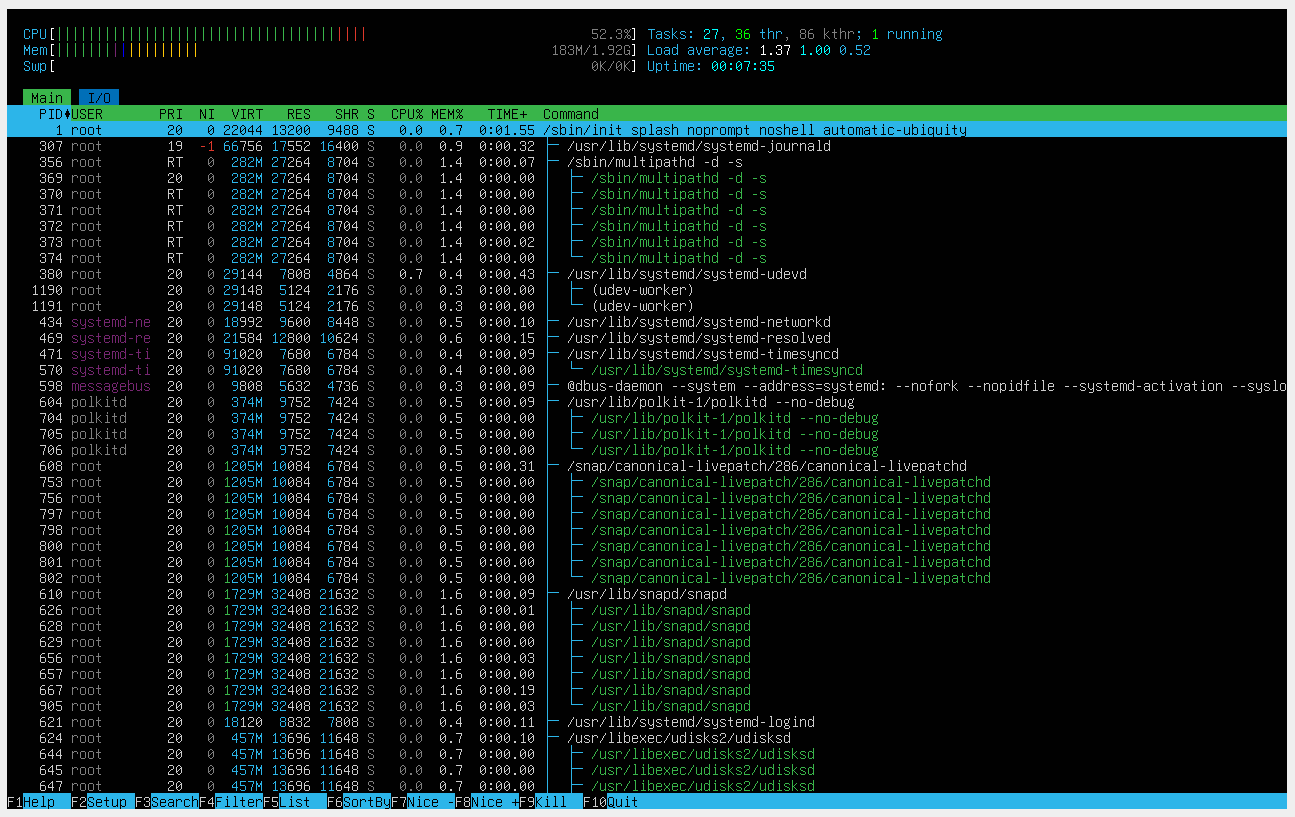
\includegraphics[width=0.8\textwidth]{./images/medcpuload.png}
    \caption{\mintinline{python}{htop} output when running \mintinline{shell}{python3 stress_cpu.py --load medium}}
\end{figure}

\begin{figure}[H]
    \centering
    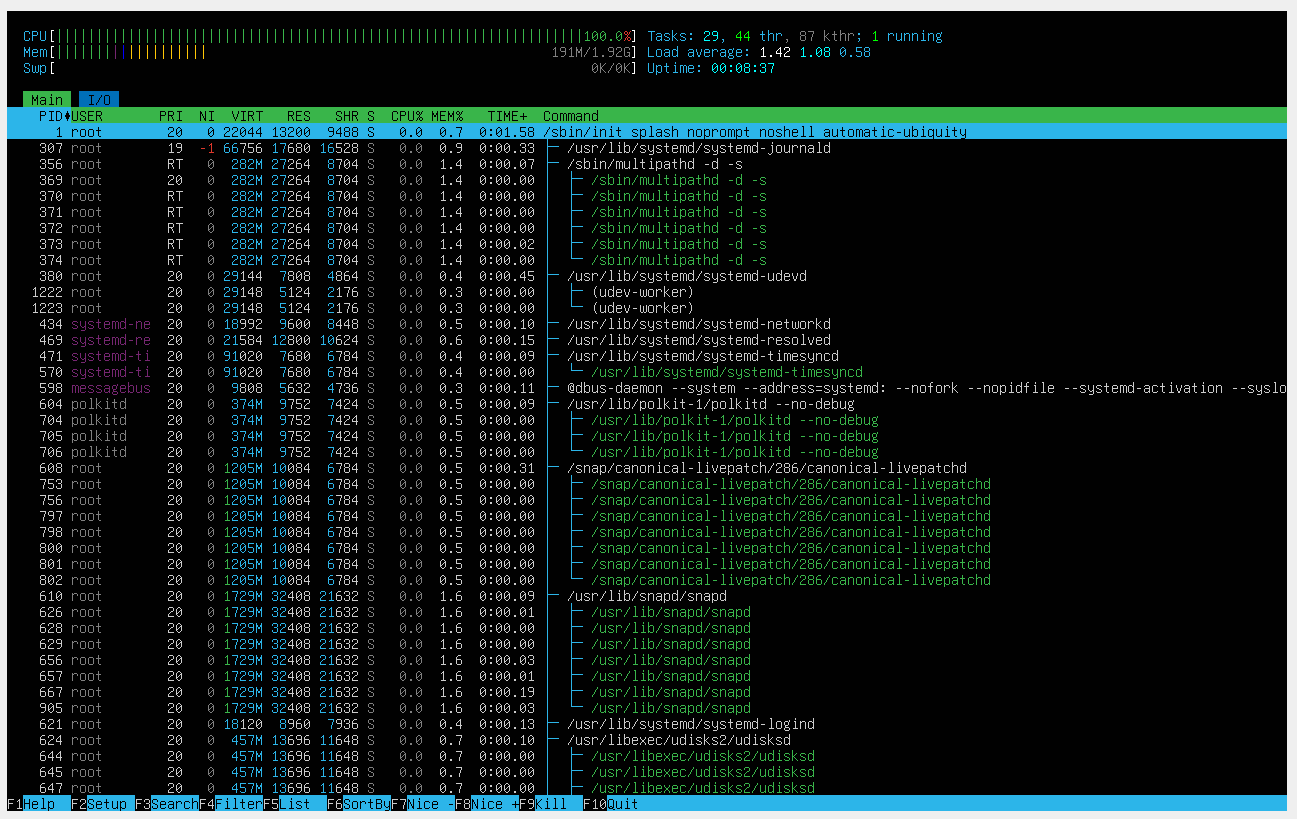
\includegraphics[width=0.8\textwidth]{./images/highcpuload.png}
    \caption{\mintinline{python}{htop} output when running \mintinline{shell}{python3 stress_cpu.py --load high}}
\end{figure}

\begin{code}
\inputminted[linenos, breaklines, frame=single]{python}{../code/stressers/stress_memory.py}
\caption{\texttt{stress\_memory.py}}
\end{code}

I found that the maximum \mintinline{shell}{--usage} value I could set without getting the process killed by the Linux kernel's Out-Of-Memory (OOM) killer was \mintinline{shell}{0.85}, so this is the value I used for my experiments.

\begin{figure}[H]
    \centering
    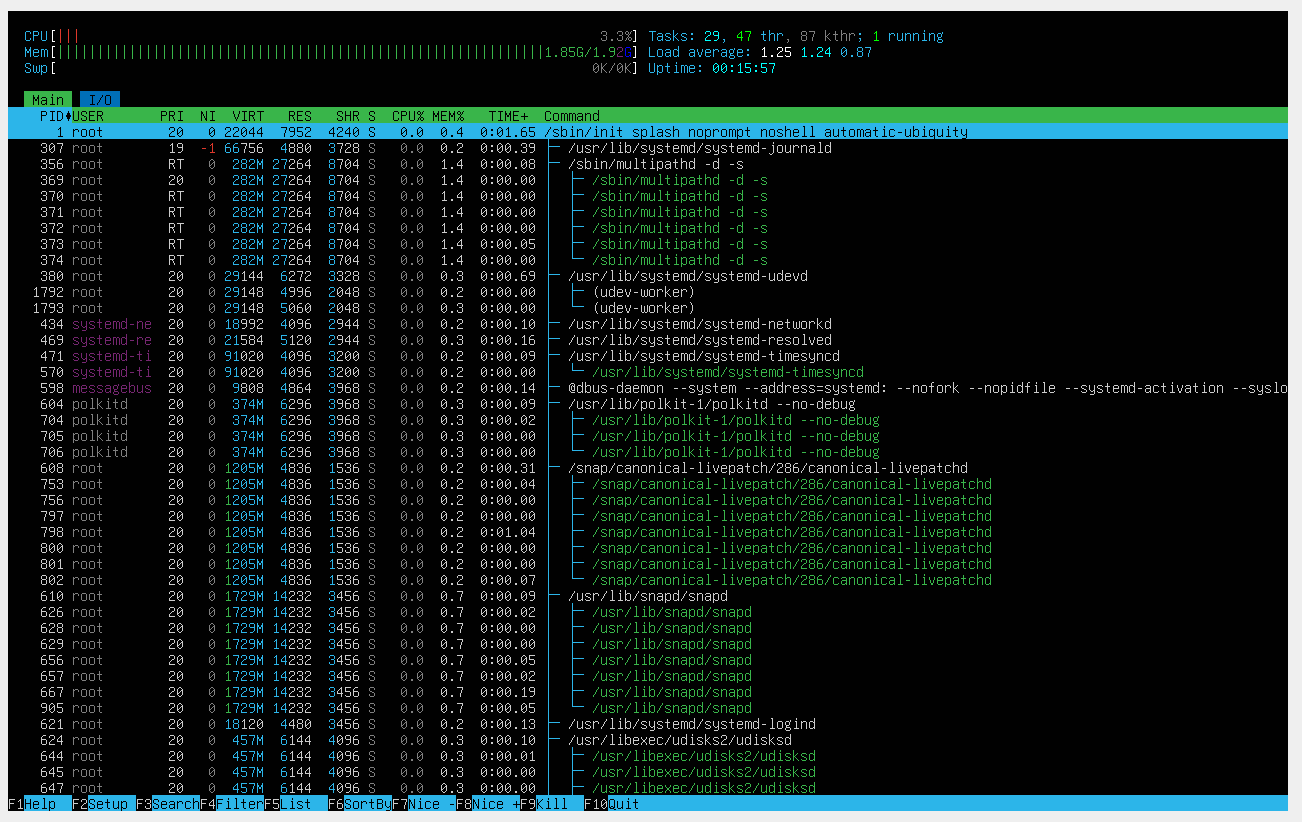
\includegraphics[width=\textwidth]{./images/memstress.png}
    \caption{\mintinline{python}{htop} output when running \mintinline{shell}{python3 stress_memory.py --usage 0.85}}
\end{figure}

\section{Experiments}
I ran the experiments in quick succession on the virtual machine by running the appropriate stresser script(s), forking it into the background using the \mintinline{shell}{&} shell operator, and running the merged benchmark program.
I then transferred the generated CSV files to my host machine using \mintinline{shell}{scp}.
To generate the plots, I wrote a Python script which will plot the mean, minimum, maximum, or standard deviation of the values collected in a bar chart for a number of given CSV files.

\begin{code}
\inputminted[linenos, breaklines, frame=single]{python}{../code/plots/barchart.py}
\caption{\texttt{barchart.py}}
\end{code}

It's important to note that the plots which display the mean value for each experiment could be misleading:
if there was a high degree of variance in the collected results, with positive \& negative values, they could cancel each other out and result in a deceptively small mean.

\subsection{Signal Handling}
The experimental data collected for the signal handling metric surprised me, as it did not match my expected results.
Since this benchmark measures the latency between sending a signal to a process and the process executing it in its signal handler function, I would expect the mean latency to increase as CPU \& memory load were increased.
As the CPU load increases, processes can be delayed in their execution due to scheduling, and processes may be preempted, causing higher latency.
I would expect high memory consumption to have similar effects, especially when memory locking is disabled, as the process data may then be swapped out, which is extremely slow \& costly.
\\\\
However, as can be seen in the figures below, this wasn't really the case for my collected data.
The variance in my charted results seem to just be artefacts of noise in the system and fluctuations in the experimental conditions, as they don't seem to follow any discernible pattern.
The main reason why I think this may have happened is because of the \verb|PREEMPT_RT| kernel patches that I installed, which turned the OS into a fully-preemptible RTS, resulting in more predictable response times, and better prioritisation of tasks;
since the benchmark program runs with maximum priority, lower priority processes like my stresser scripts could get preempted in favour of the high priority benchmarking program, thus resulting in the benchmarking program not being majorly effected by the system load.
\\\\
I found these results very surprising, but upon reflection, they make sense, and are indicative of the power of the Linux kernel for use in hard RTS applications when the \verb|PREEMPT_RT| patches are applied.

\begin{figure}[H]
    \centering
    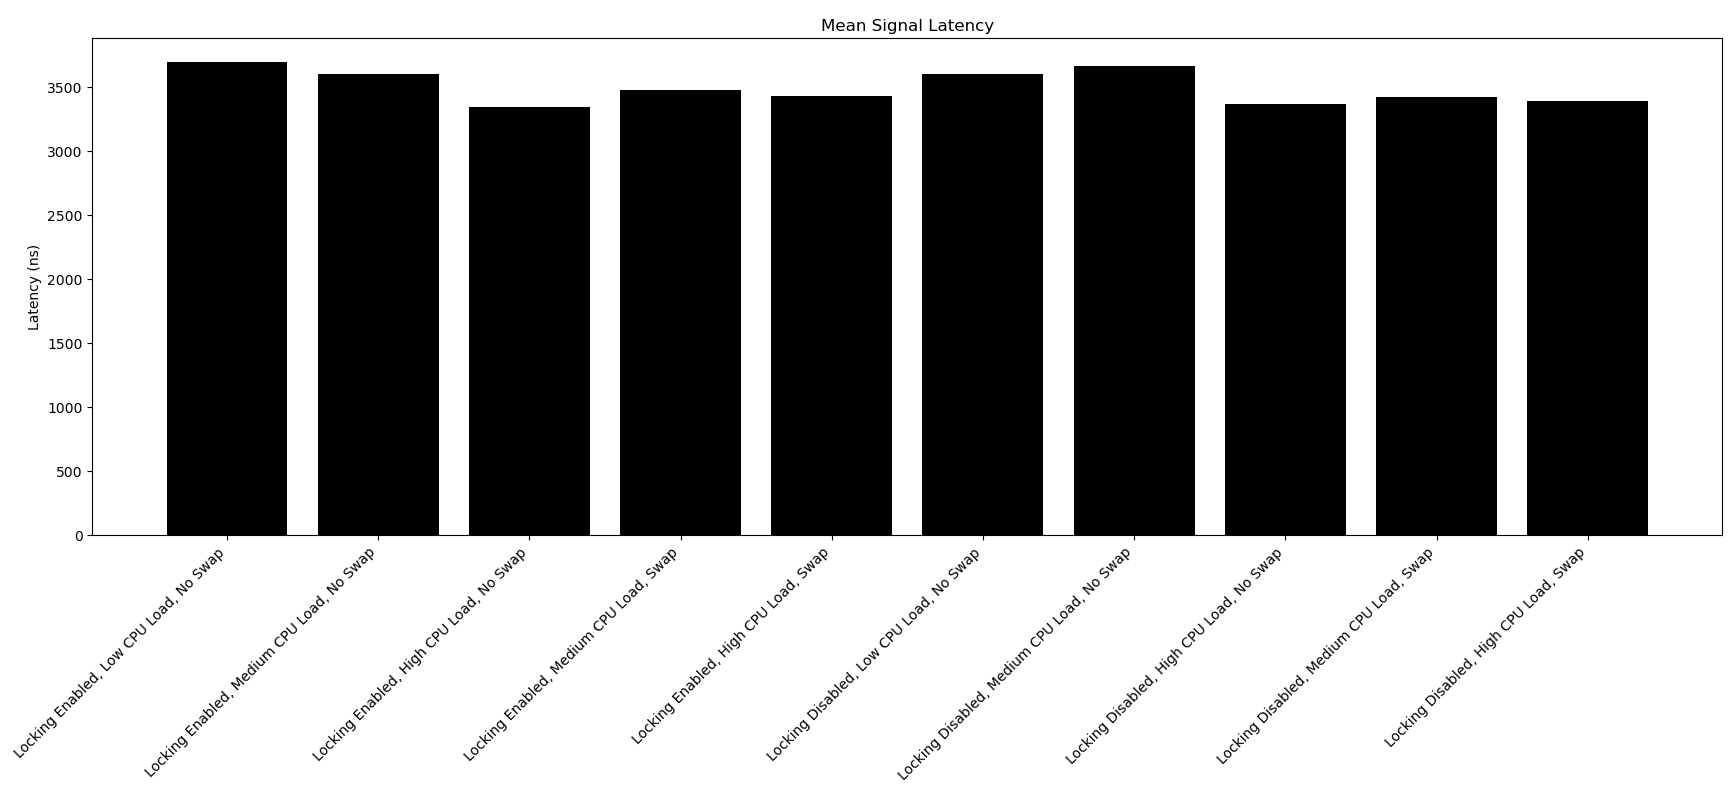
\includegraphics[width=\textwidth]{./images/signal-mean.png}
    \caption{Mean latency for the signal handling benchmark}
\end{figure}

\begin{figure}[H]
    \centering
    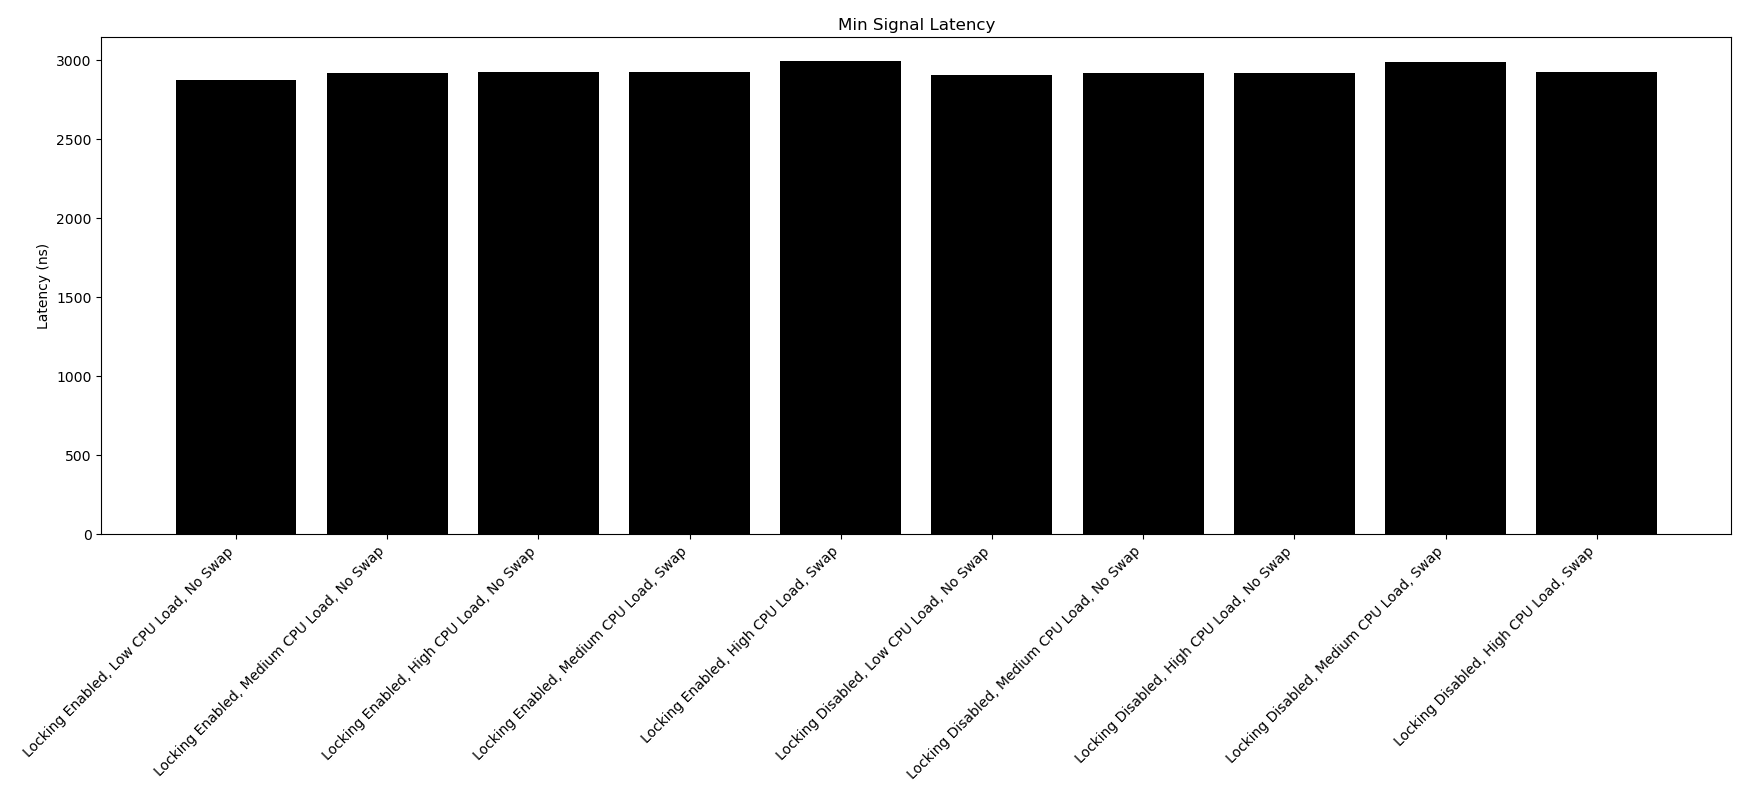
\includegraphics[width=\textwidth]{./images/signal-min.png}
    \caption{Minimum latency for the signal handling benchmark}
\end{figure}

\begin{figure}[H]
    \centering
    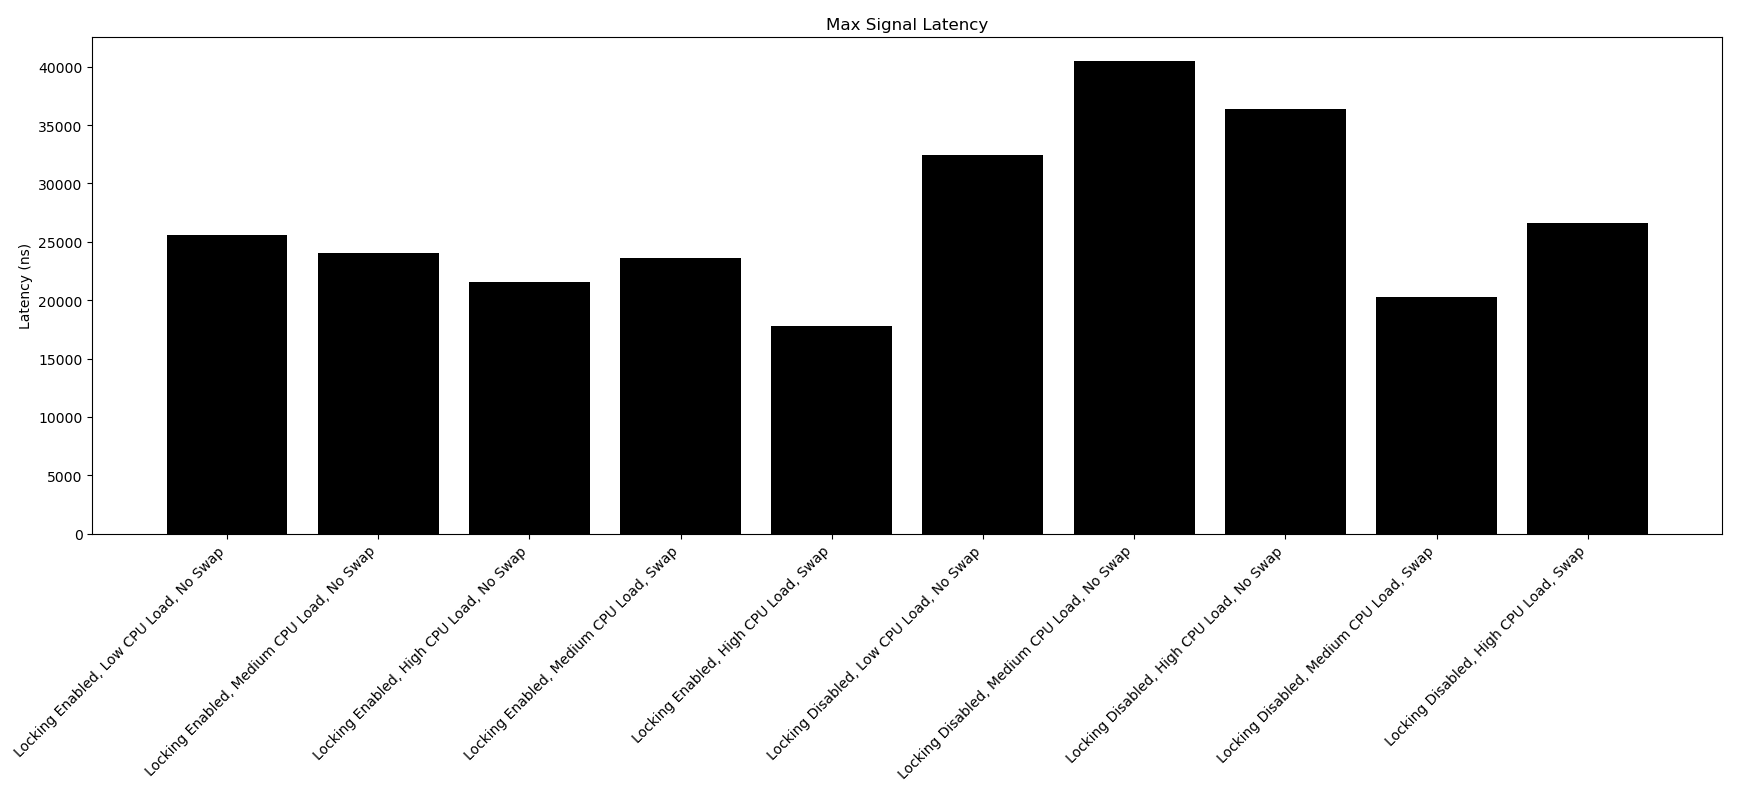
\includegraphics[width=\textwidth]{./images/signal-max.png}
    \caption{Maximum latency for the signal handling benchmark}
\end{figure}

\begin{figure}[H]
    \centering
    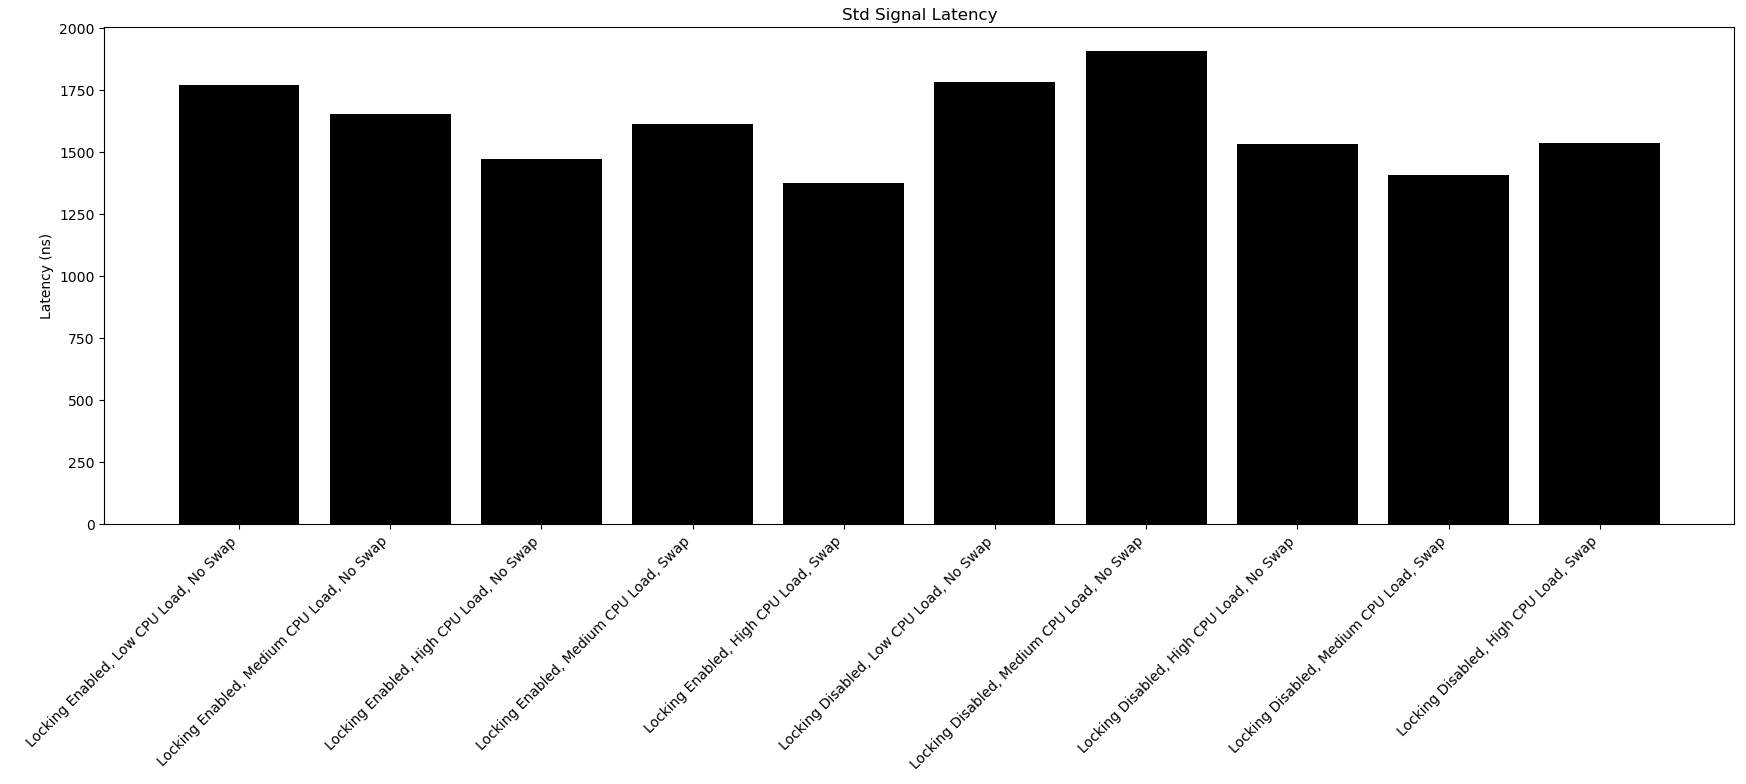
\includegraphics[width=\textwidth]{./images/signal-std.png}
    \caption{Standard deviation of latency for the signal handling benchmark}
\end{figure}

\subsection{Interval Timer}
Since the interval timer benchmark uses a POSIX interval timer to trigger a signal at precise intervals, I would expect the time interrupts to be precisely scheduled under low CPU load, and greater delay to appear under higher CPU load due to the CPU being busy. 
I would also expect swapping to worsen the jitter, as accessing the memory will be in the order of milliseconds rather than microseconds.
However, as previously discussed, the \verb|PREEMPT_RT| patches will help to mitigate these issues.
We can see from the output data that, while not a clean trend upwards, there tends to be a higher jitter value for higher CPU loads.
The most telling metric is the standard deviation;
we can see from the standard deviation plot below that the variance in jitter trends upwards as CPU load \& memory load increase, as one would expect.

\begin{figure}[H]
    \centering
    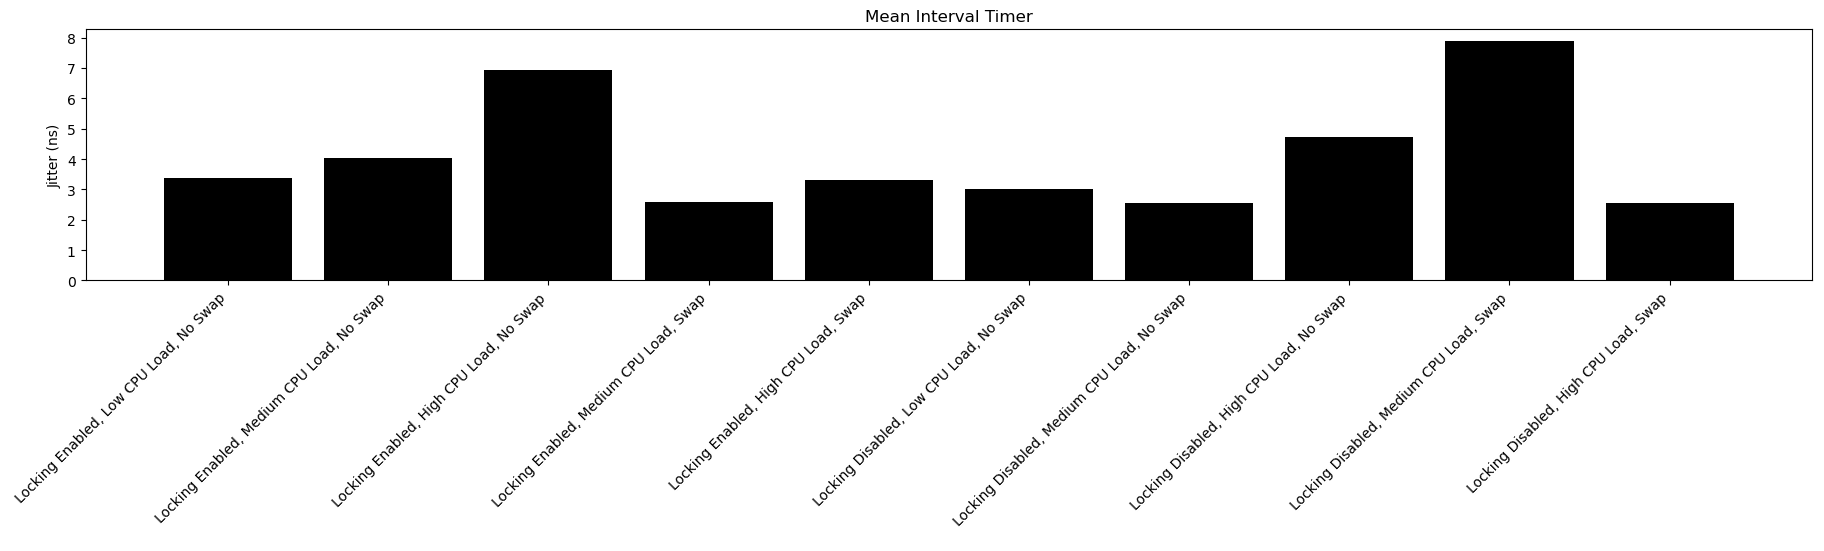
\includegraphics[width=\textwidth]{./images/interval-mean.png}
    \caption{Mean jitter for the interval timer benchmark}
\end{figure}

\begin{figure}[H]
    \centering
    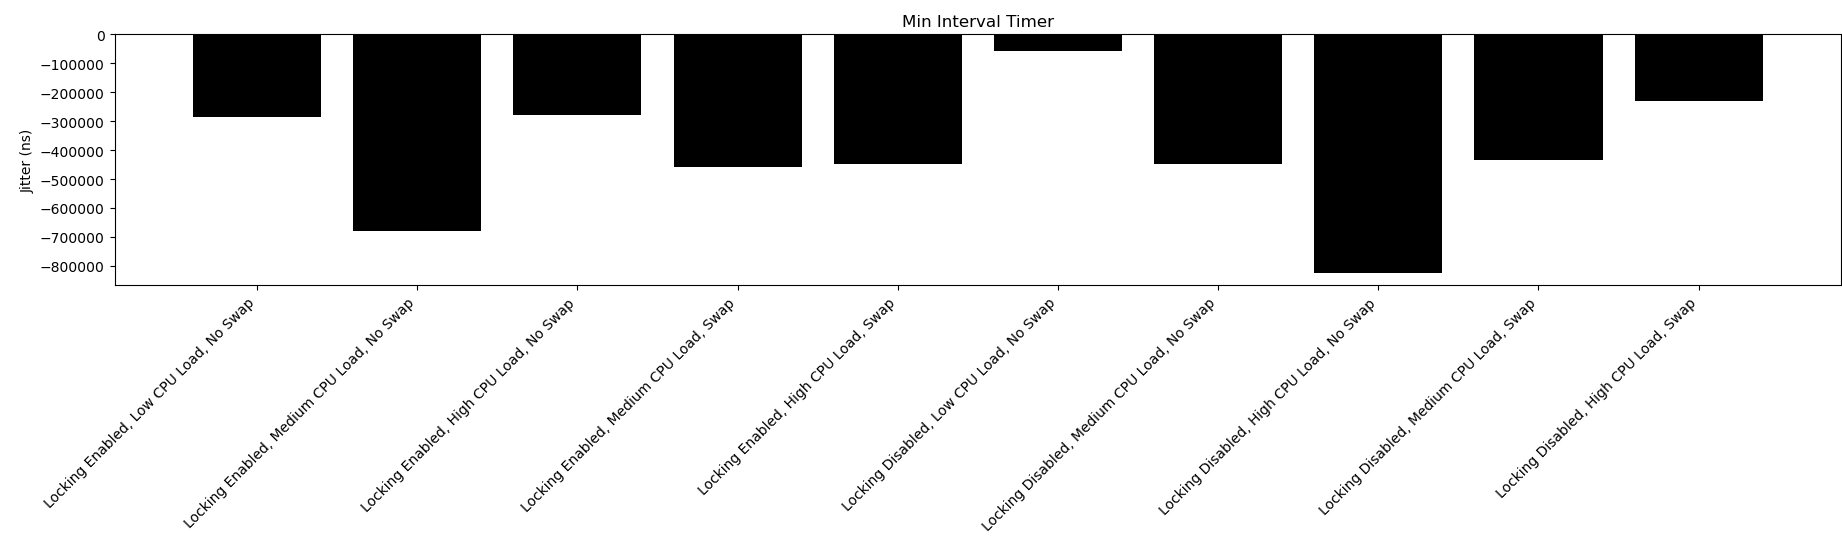
\includegraphics[width=\textwidth]{./images/interval-min.png}
    \caption{Minimum jitter for the interval timer benchmark}
\end{figure}

\begin{figure}[H]
    \centering
    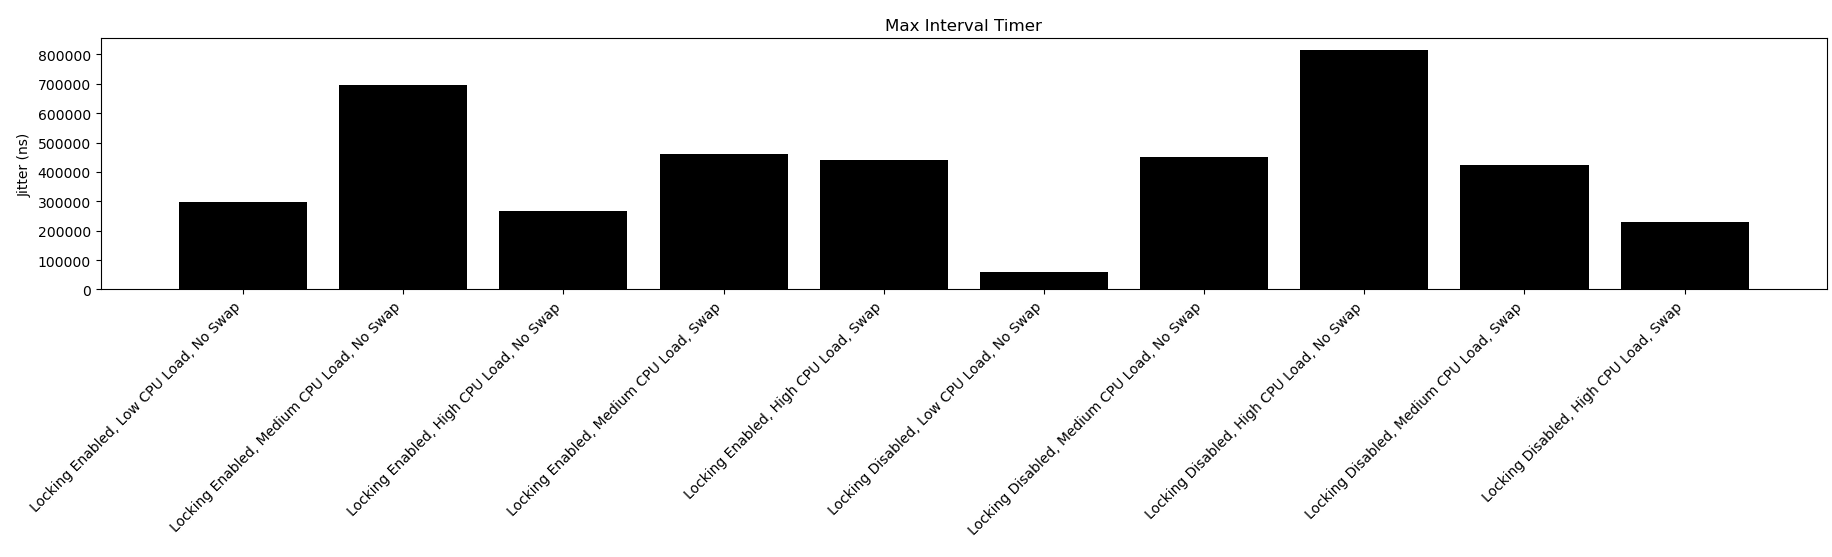
\includegraphics[width=\textwidth]{./images/interval-max.png}
    \caption{Maximum jitter for the interval timer benchmark}
\end{figure}

\begin{figure}[H]
    \centering
    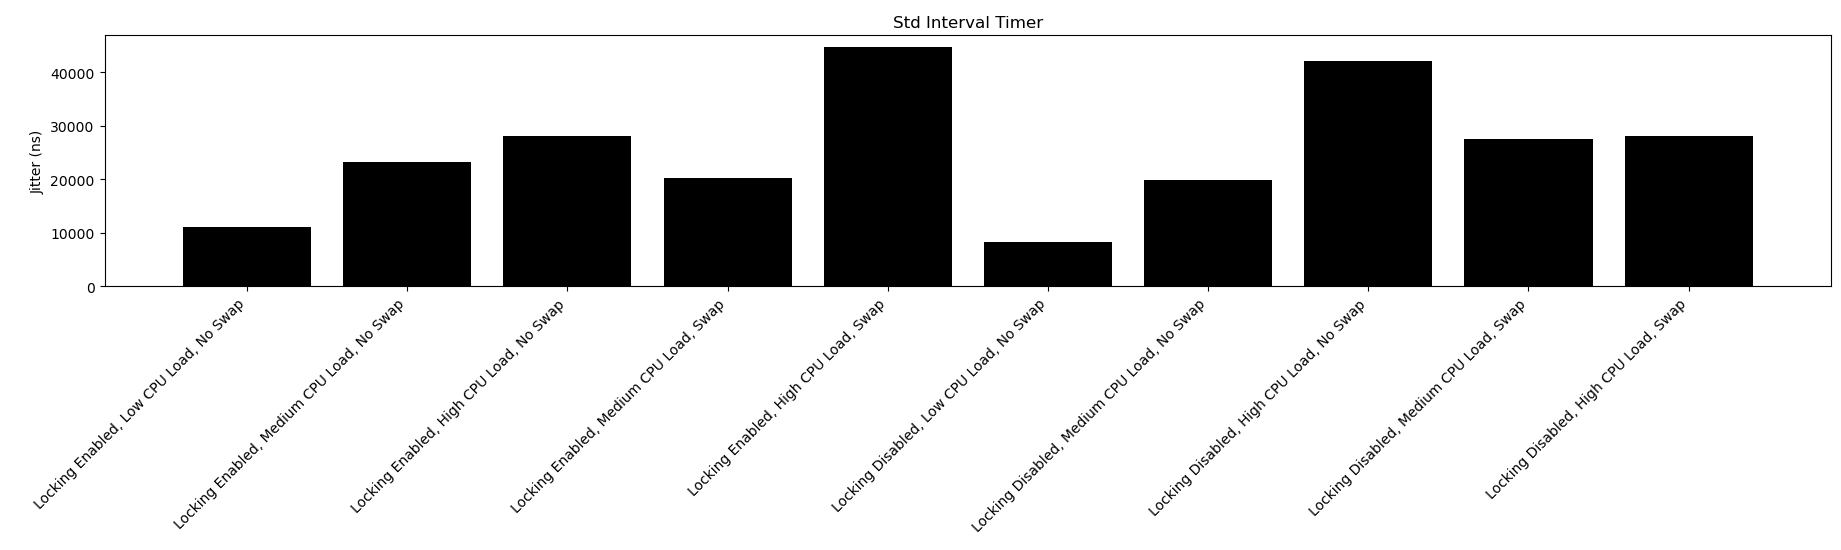
\includegraphics[width=\textwidth]{./images/interval-std.png}
    \caption{Standard deviation of jitter for the interval timer benchmark}
\end{figure}


\subsection{\mintinline{c}{nanosleep()}}
Since the \mintinline{c}{nanosleep()} benchmark measures the actual time elapsed versus the requested sleep duration, we would expect it to increase as the CPU load increases due to scheduling latency inducing jitter.
Memory swapping adds large delays, and one would expect high CPU and high swap to cause erratic \& unpredictable behaviour, making sleep times unreliable.
The application of the \verb|PREEMPT_RT| patches should increase the accuracy of sleep times, as the wake-ups will happen closer to the requested sleep duration and result in a lower maximum jitter value as the process can preempt other lower-priority tasks.
The plotted charts don't bear a great deal of resemblance to the expected results, which is likely in large part due to the \verb|PREEMPT_RT| patches, but also likely due to the large number of background tasks that are running at a given time on an Ubuntu system, which could be introducing noise into the data.

\begin{figure}[H]
    \centering
    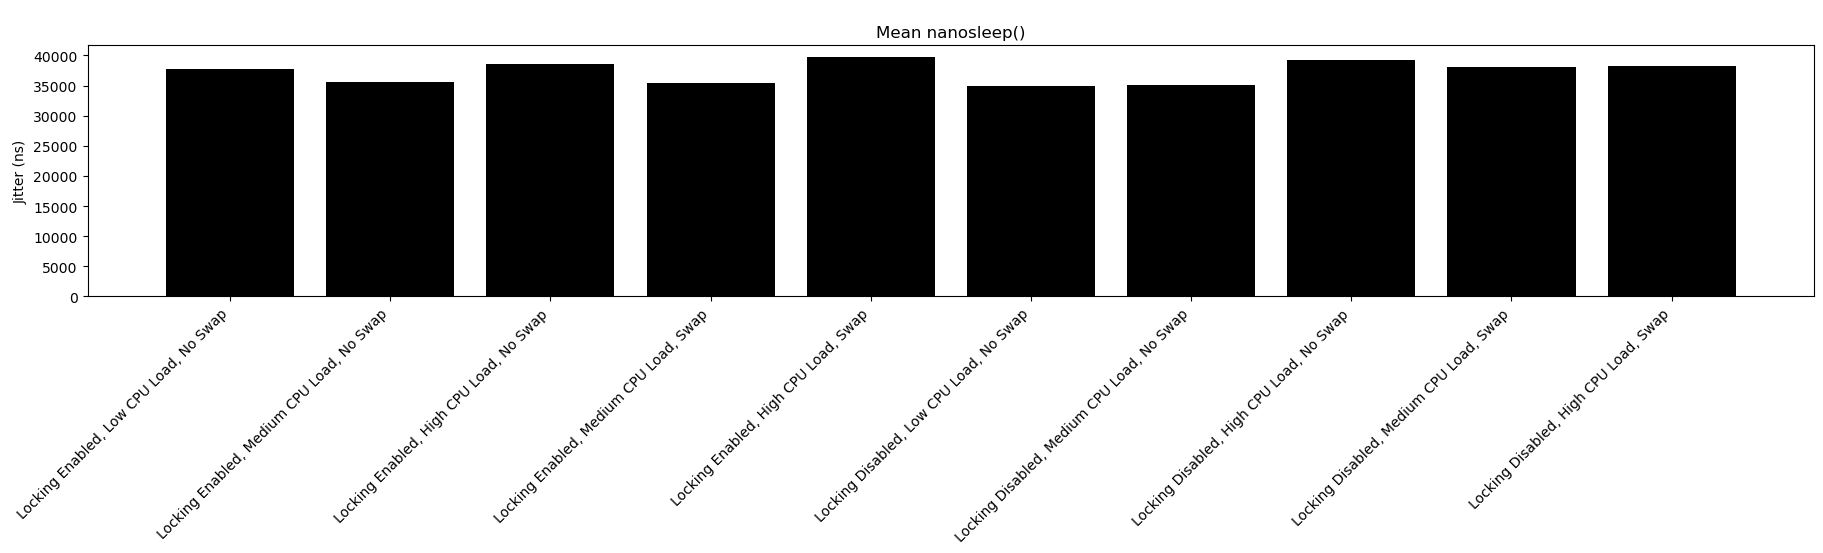
\includegraphics[width=\textwidth]{./images/nanosleep-mean.png}
    \caption{Mean jitter for the \mintinline{c}{nanosleep()} benchmark}
\end{figure}

\begin{figure}[H]
    \centering
    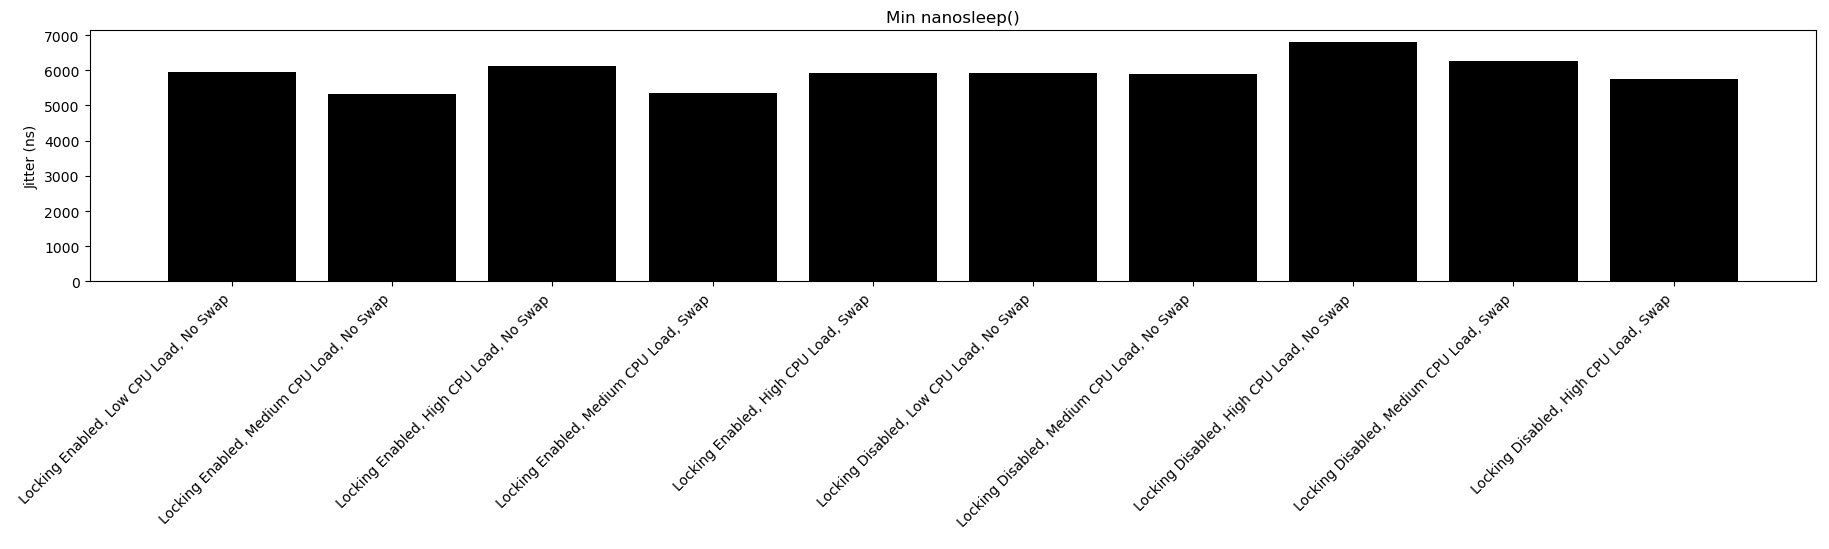
\includegraphics[width=\textwidth]{./images/nanosleep-min.png}
    \caption{Minimum jitter for the \mintinline{c}{nanosleep()} benchmark}
\end{figure}

\begin{figure}[H]
    \centering
    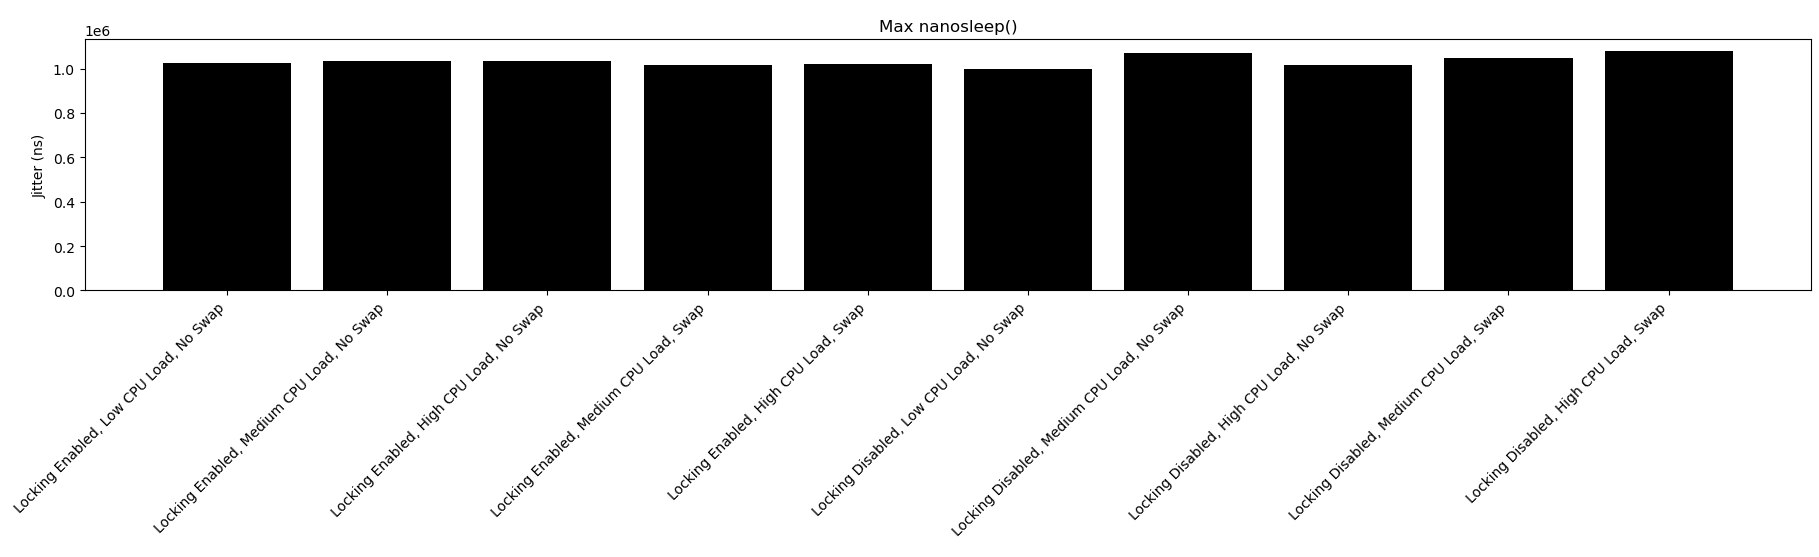
\includegraphics[width=\textwidth]{./images/nanosleep-max.png}
    \caption{Maximum jitter for the \mintinline{c}{nanosleep()} benchmark}
\end{figure}

\begin{figure}[H]
    \centering
    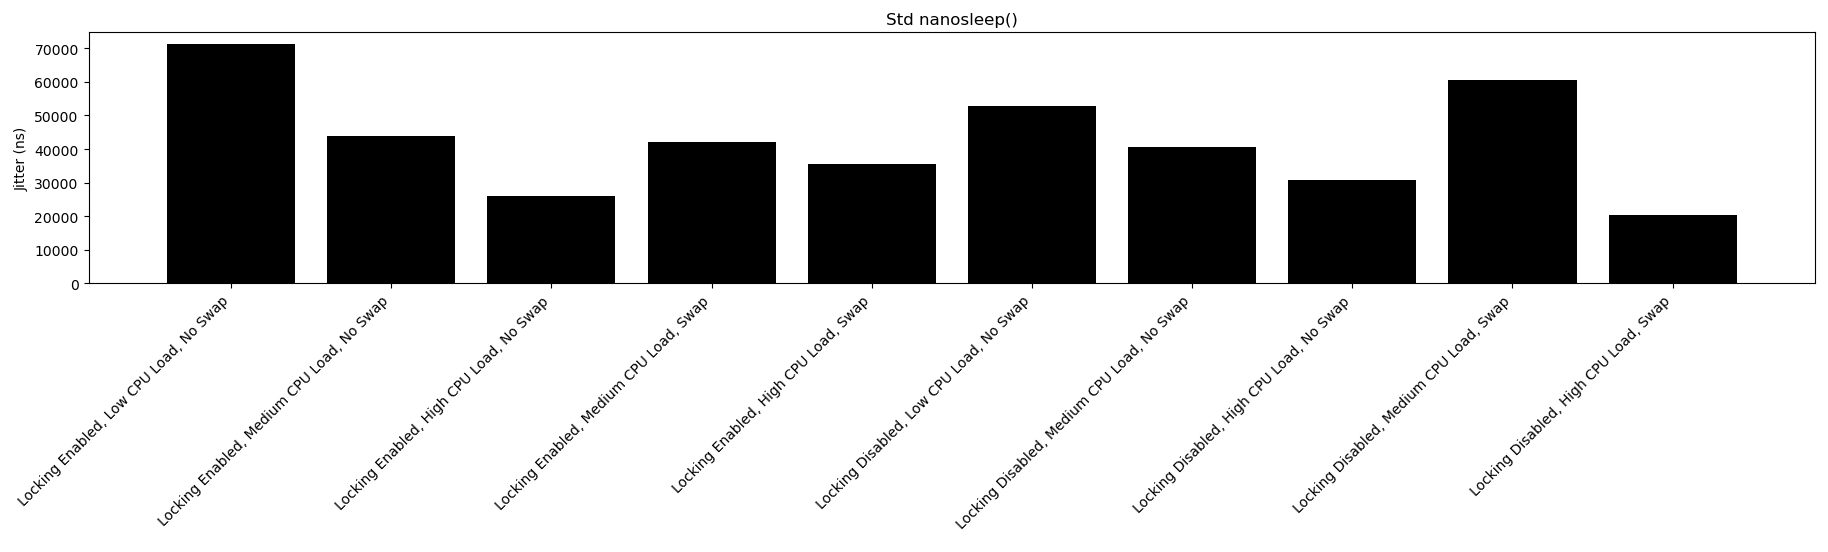
\includegraphics[width=\textwidth]{./images/nanosleep-std.png}
    \caption{Standard deviation of jitter for the \mintinline{c}{nanosleep()} benchmark}
\end{figure}

\subsection{\mintinline{c}{usleep()}}
The \mintinline{c}{usleep()} function serves a similar role to \mintinline{c}{nanosleep()}, with the primary difference being that \mintinline{c}{usleep()} has precision in the microseconds (the \verb|u| is an ASCII approximation of the $\mu$ symbol typically used to symbolise the ``micro'' prefix) rather than in the nanoseconds, and is thus far less precise.
For this reason, greater jitter is to be expected.
At low CPU usage, we would expect slightly worse performance than \mintinline{c}{nanosleep()}, and for this performance to decrease as CPU usage increases;
similar behaviour is to be expected as memory usage increases also.
Since \mintinline{c}{usleep()} relies on signals internally, it could potentially suffer more greatly under high CPU strain.  
The \verb|PREEMPT_RT| patches can help to improve response times due to the preemptible kernel, but swapping will still cause performance issues.
\\\\
The most interesting plot for this benchmark is the standard deviation plot below, as it corresponds pretty much exactly to what we would expect; clearly, \mintinline{c}{usleep()} derives less performance benefit from \verb|PATCHES_RT| than \mintinline{c}{nanosleep()}.
The jitter is lowest when locking is enabled, there is low CPU load, and no swap, and increases as the CPU load \& memory load are increased.
When locking is disabled, there is greater performance degradations between the low CPU/memory experiment and the subsequent experiments, with the high CPU, high memory, no locking experiment yielding the greatest standard deviation, and thus the least predictability.

\begin{figure}[H]
    \centering
    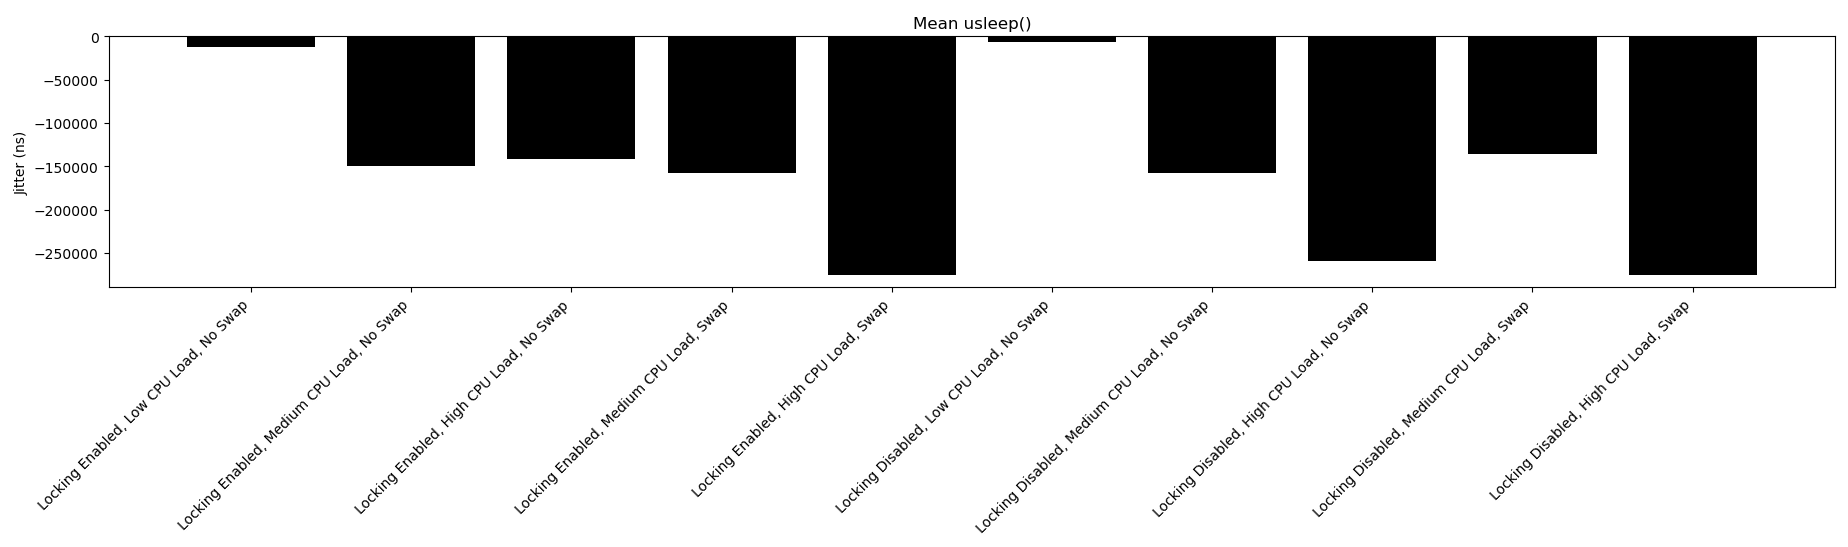
\includegraphics[width=\textwidth]{./images/usleep-mean.png}
    \caption{Mean jitter for the \mintinline{c}{usleep()} benchmark}
\end{figure}

\begin{figure}[H]
    \centering
    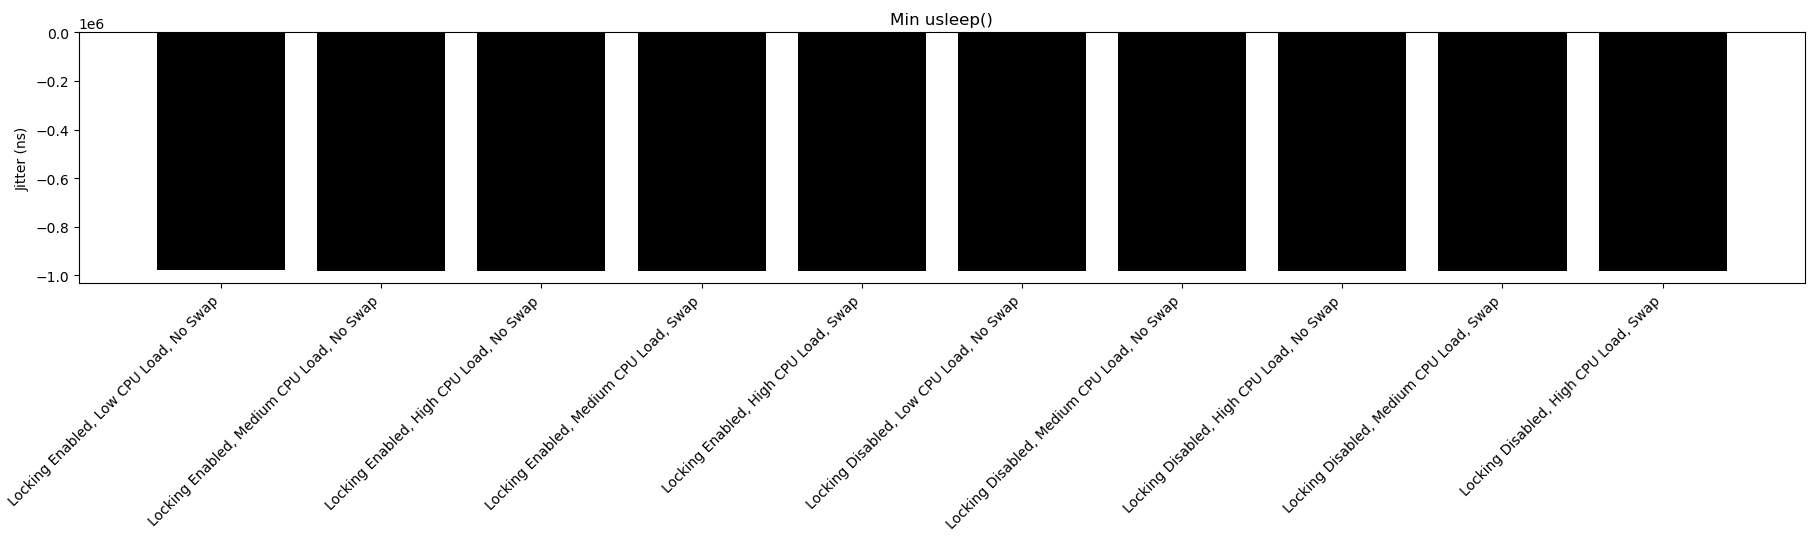
\includegraphics[width=\textwidth]{./images/usleep-min.png}
    \caption{Minimum jitter for the \mintinline{c}{usleep()} benchmark}
\end{figure}

\begin{figure}[H]
    \centering
    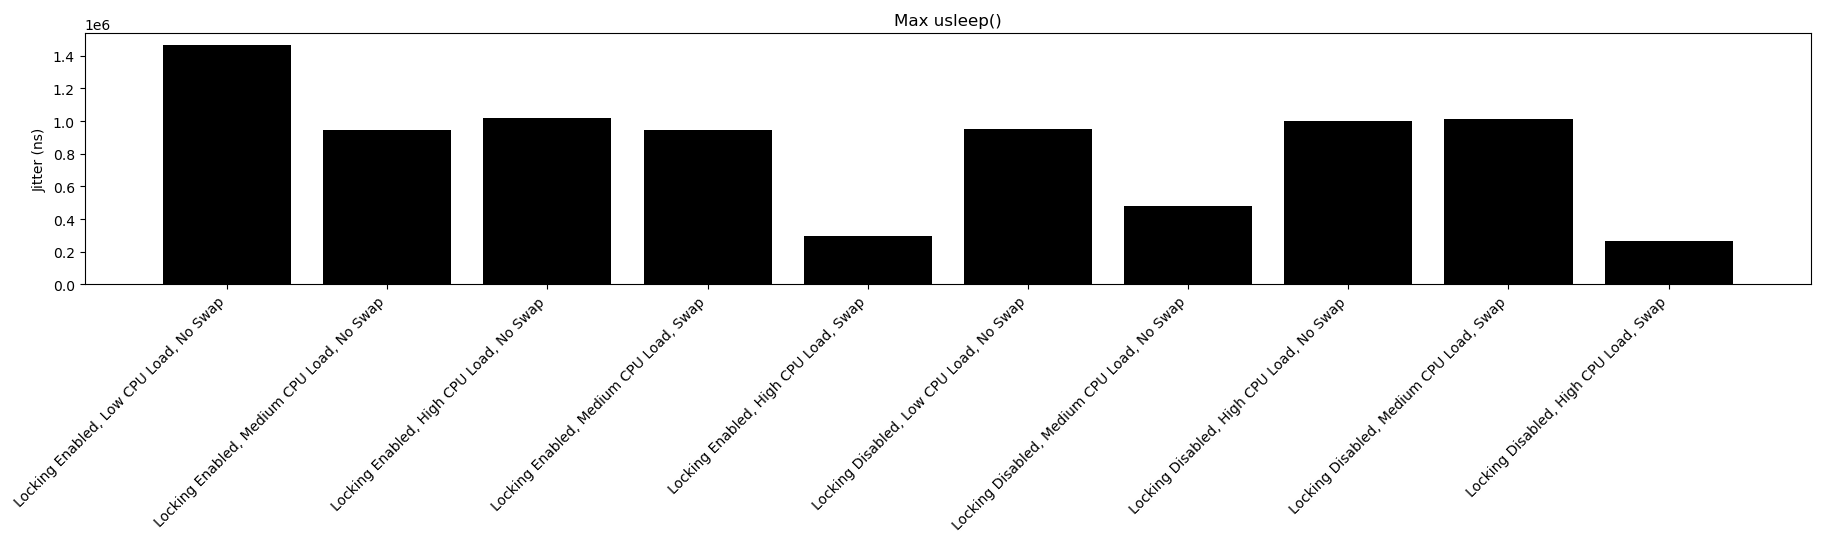
\includegraphics[width=\textwidth]{./images/usleep-max.png}
    \caption{Maximum jitter for the \mintinline{c}{usleep()} benchmark}
\end{figure}

\begin{figure}[H]
    \centering
    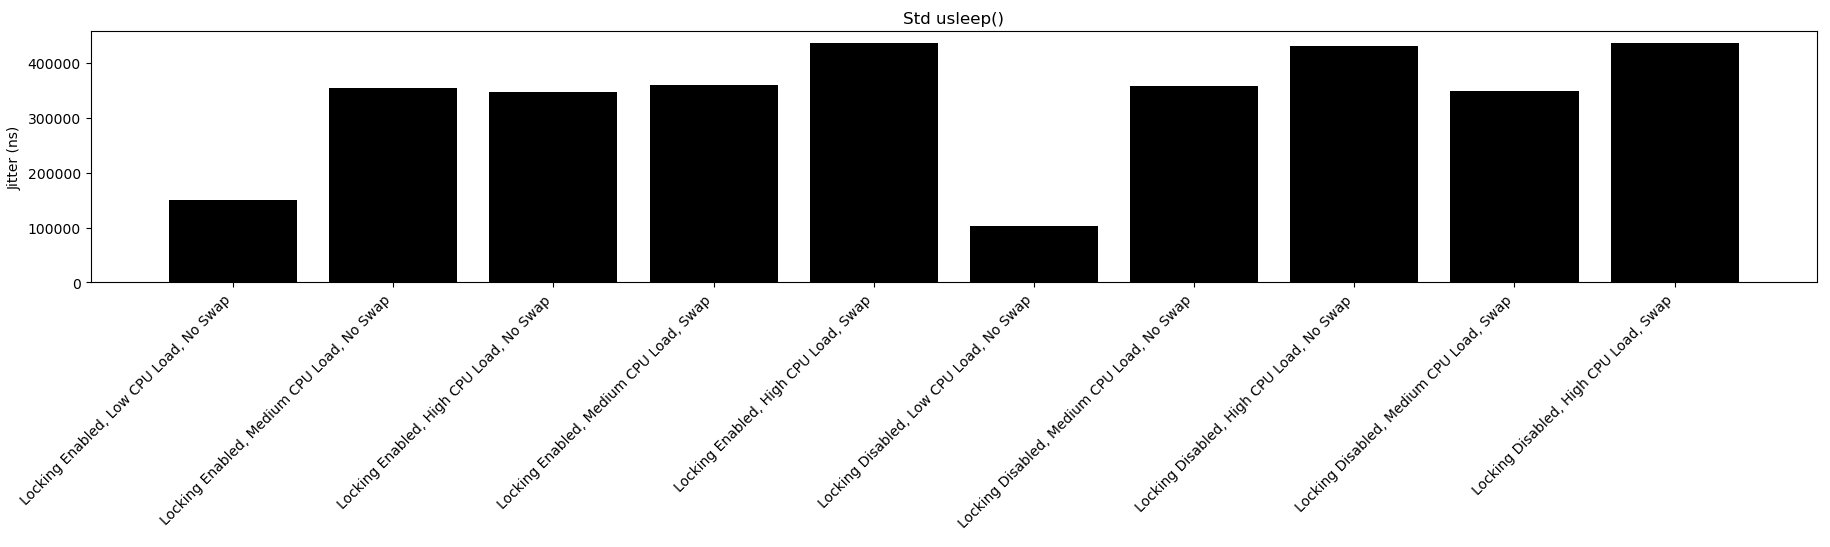
\includegraphics[width=\textwidth]{./images/usleep-std.png}
    \caption{Standard deviation of jitter for the \mintinline{c}{usleep()} benchmark}
\end{figure}

\section{Conclusions}
To conclude, as CPU load \& memory load increase, performance in terms of jitter \& latency are to be expected to degrade.
Memory locking helps to mitigate the negative effects of high memory consumption, by preventing the memory from being swapped.
Using a fully preemptible kernel like the Linux kernel with the \verb|PREEMPT_RT| patches applied can limit the negative effects of system strain, and help to ensure that deadlines are met, making such kernels a good choice for any kind of RTS, but particularly hard real-time systems.

\printbibliography

\end{document}
